\section{Design}

The design goals of NVKV are five-fold:
\begin{enumerate}
	\item \textbf{Direct Access}: BNVM should be operated on \textit{directly},
		without operating system interposition and without additional copies, as
		much as possible. This is possible in Linux using BNVM drivers and DAX
		\texttt{mmap}~\cite{dax}, wherein an application can memory map the
		actual BNVM directly into its address space.
	\item \textbf{Consistency with Operations}: Once each operation returns to
		the application, any changes required by the operation must be
		persistent. For example, after the insert function returns, the new data
		and the updated information in the index must be persisted to BNVM such
		that if power failed at that point, the insert operation would be safe.
	\item \textbf{Consistency with Power Failures}: NVKV must support power
		failures at \textit{any} point during \textit{any} operation. When power
		is resumed, and the application restarted, it should be able to continue
		operating without the database having been corrupted. In this case, we
		define free from corruption as all values that were inserted can be
		found, all items that were deleted cannot be found, all data that was in
		the database remains the same across power failures, and keys and values
		match as expected.

		If a power failure occurs in the middle of an insert, there is a
		possibility that the insert only partially completely. That is fine, as
		long as the above requirements are met. For example, the data might be
		copied in before the index is updated. If the power fails here, the only
		``inconsistency'' would be that there is a key-value pair that is not
		retrievable, which does not violate the above requirements because the
		insert operation had not yet returned to the user. However, this
		database state is sub-optimal since it contains unnecessary data. For
		these kinds up inconsistencies, we allow a fsck tool to be run to
		measure reachability for all keys and values and ensure that the
		database count is correct. Note that if the database was used without
		running the fsck tool, it would work as expected; the fsck tool is just
		there to optimize the database when power failures occur.
	\item \textbf{Performance}: Like any good key-value store, NVKV aims to
		provide the design requirements while being high performance.
		Specifically, it aims to be \textit{low-latency} to match the
		low-latency access to persistent storage that BNVM provides.
	\item \textbf{Compatibility}: To ease evaluation, NVKV provides an identical
		interface to Berkeley DB. When developing a new system, adoption is key,
		and backwards compatibility is vital for increasing adoption.
\end{enumerate}

Common themes: small sub-operations, avoid movement.

Limits of transactions... "when I say transaction i refer to a mem transaction"

\subsection{Interface}

The interface to applications provided by NVKV is just like Berkeley DB. In
fact, the only difference is in the header file that must be included by the
application (\texttt{db.h} in the case of \bdb and \texttt{nvkv.h} in the case
of NVKV). Applications then link with \texttt{libnvkv.so}. The interfaces are
exactly the same, although a lot of functionality is left unimplemented, as full
compatibility is well outside the scope of a class project. The implemented
functionality is \texttt{db\_create}, \texttt{db\_open}, \texttt{get},
\texttt{put}, \texttt{sync}, \texttt{err}, \texttt{errx}, and manipulation of
\texttt{DBT}s. The format of the database files is \textit{not} compatible; only
the programming interface is.

\subsection{Data Organization}

The database file contains two separate types of data: data and metadata. Data
refers to the contents of a \texttt{DBT} (keys and values) along with their
lengths. The exact format of the data storage is discussed in
section~\ref{sec:ds}. Metadata is the information kept by the database in order
to support the lookup operations on the data; that is, a small structure
containing information about the database as a whole, and the indexing data
structure.

\begin{figure}
\centering
\hspace*{-0.1in}
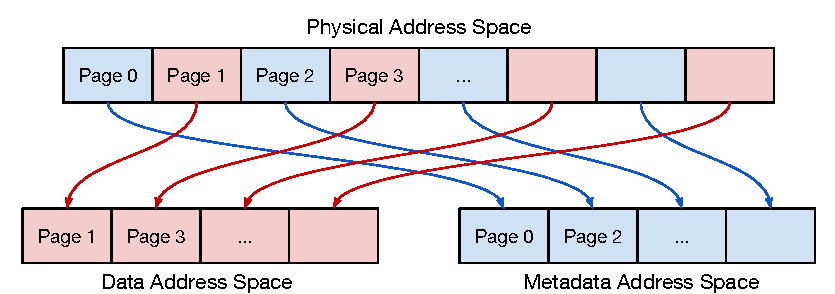
\includegraphics[width=84mm]{fig/addrspace}
\caption{Mapping the data and metadata address spaces to the physical address
space of the database file.}
\label{fig:addrspace}
\end{figure}

Since NVKV maintains backwards compatibility with \bdb, it is allowed only one file to
store both metadata and data. However, both of these grow when inserting,
meaning that if they were placed naively inside the database file, they might
have to be moved. Moving large amounts of data is fine in a database system
such as \bdb, but when operating directly on BNVM, we must avoid moving data
when possible. Furthermore, moving data is much more difficult to do in a single
transaction.

To avoid moving data, NVKV lays out memory as shown in
figure~\ref{fig:addrspace}, where each page of metadata is interlaced with each
data page. Logically, this provides two separate, linear address spaces for data
and metadata. Internal pointers are stored \textit{as if} these address spaces
were real and started at zero; that is, if page-size is 4K and we wished to
write a pointer to the second page of metadata, it would be \texttt{0x1000 +
page-offset}, even though the actual location in the file this refers to is
\texttt{0x2000 + page-offset}. When swizzling pointers into their virtual
address space value after \texttt{mmap}ing the database, NVKV relies on context
to choose the address space, apply the appropriate operation to determine the
offset into the file, and then adds the base address of the \texttt{mmap}
region to calculate the ultimate virtual address.

The need to deal with persistent pointers in virtual memory is a real problem,
because we can no longer have an explicit serialization step when persisting to
persistent memory---after all, the data is already persistent. Thus, we must
always write pointers to memory in a universal format that applications can make
use of regardless of the ultimately mapped location of the data that is pointed
to or the pointers themselves. We are working on a larger project named
Twizzler~\cite{bittman-ssrctr-17-01} that addresses and explores these issues in
detail and provides a programming model based around transparent use of
universal pointers. If that system was fully functional, most of the complexity in this
key-value store would be trivial, since most of the code complexity comes from
dealing with swizzling between these different address spaces (data, metadata,
persistent, and virtual).


\subsection{Indexing}

\subsection{Data Storage}
\label{sec:ds}

\subsection{Transaction Sizes}

Key points: transactions have limited size, both in space and time. A
transaction cannot take too many instructions, nor have too many memory
accesses. Of course, we're designing under an assumption about how transactions
will work... they may turn out differently. So we're designing pessimistically.

num memory accesses matter more than number of instructions, but the total length
matters too.

We can also optimize certain parts of the code with Os and other parts with
O2/3.












\begin{figure}
\centering
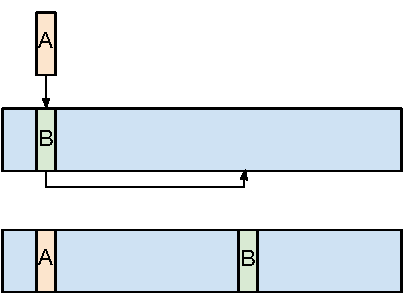
\includegraphics[width=70mm,height=50mm]{fig/cuckoo_insert}
\caption{Inserting an element that requires moving an existing element to a
partner bucket.}
\label{fig:insert}
\end{figure}

\begin{figure}
\centering
\hspace*{1mm}
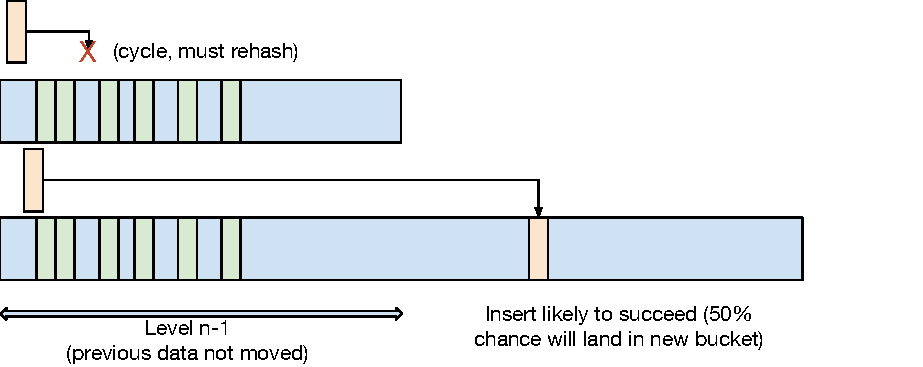
\includegraphics[width=100mm]{fig/cuckoo_rehash}
\caption{Extending the hash table to level $n$ without reinserting existing
elements. Level $n-1$ has existing elements that are not moved during the
expansion, and the newly inserted element is more than twice as likely to find
an empty bucket to insert into.}
\label{fig:rehash}
\end{figure}

